%%%%%%%%%%%%%%%%%%%%%%%%%%%%%%%%%%%%%%%%%
% Playbook
% Panos Lab Methodologies
% by Matt Green
%%%%%%%%%%%%%%%%%%%%%%%%%%%%%%%%%%%%%%%%%

%----------------------------------------------------------------------------------------
%	PACKAGES AND OTHER DOCUMENT CONFIGURATIONS
%----------------------------------------------------------------------------------------

\documentclass{tufte-book} % Use the tufte-book class which in turn uses the tufte-common class

\hypersetup{colorlinks} % Comment this line if you don't wish to have colored links

\usepackage{microtype} % Improves character and word spacing

\usepackage{lipsum} % Inserts dummy text

\usepackage{booktabs} % Better horizontal rules in tables

\usepackage{graphicx} % Needed to insert images into the document
\graphicspath{{graphics/}} % Sets the default location of pictures
\setkeys{Gin}{width=\linewidth,totalheight=\textheight,keepaspectratio} % Improves figure scaling

\usepackage{fancyvrb} % Allows customization of verbatim environments
\fvset{fontsize=\normalsize} % The font size of all verbatim text can be changed here

\newcommand{\hangp}[1]{\makebox[0pt][r]{(}#1\makebox[0pt][l]{)}} % New command to create parentheses around text in tables which take up no horizontal space - this improves column spacing
\newcommand{\hangstar}{\makebox[0pt][l]{*}} % New command to create asterisks in tables which take up no horizontal space - this improves column spacing

\usepackage{xspace} % Used for printing a trailing space better than using a tilde (~) using the \xspace command

\newcommand{\monthyear}{\ifcase\month\or January\or February\or March\or April\or May\or June\or July\or August\or September\or October\or November\or December\fi\space\number\year} % A command to print the current month and year

\newcommand{\openepigraph}[2]{ % This block sets up a command for printing an epigraph with 2 arguments - the quote and the author
\begin{fullwidth}
\sffamily\large
\begin{doublespace}
\noindent\allcaps{#1}\\ % The quote
\noindent\allcaps{#2} % The author
\end{doublespace}
\end{fullwidth}
}

%\newcommand{\blankpage}{\newpage\hbox{}\thispagestyle{empty}\newpage} % Command to insert a blank page

\usepackage{units} % Used for printing standard units

\newcommand{\hlred}[1]{\textcolor{Maroon}{#1}} % Print text in maroon
\newcommand{\hangleft}[1]{\makebox[0pt][r]{#1}} % Used for printing commands in the index, moves the slash left so the command name aligns with the rest of the text in the index 
\newcommand{\hairsp}{\hspace{1pt}} % Command to print a very short space
\newcommand{\ie}{\textit{i.\hairsp{}e.}\xspace} % Command to print i.e.
\newcommand{\eg}{\textit{e.\hairsp{}g.}\xspace} % Command to print e.g.
\newcommand{\na}{\quad--} % Used in tables for N/A cells
\newcommand{\measure}[3]{#1/#2$\times$\unit[#3]{pc}} % Typesets the font size, leading, and measure in the form of: 10/12x26 pc.
\newcommand{\tuftebs}{\symbol{'134}} % Command to print a backslash in tt type in OT1/T1

\providecommand{\XeLaTeX}{X\lower.5ex\hbox{\kern-0.15em\reflectbox{E}}\kern-0.1em\LaTeX}
\newcommand{\tXeLaTeX}{\XeLaTeX\index{XeLaTeX@\protect\XeLaTeX}} % Command to print the XeLaTeX logo while simultaneously adding the position to the index

\newcommand{\doccmdnoindex}[2][]{\texttt{\tuftebs#2}} % Command to print a command in texttt with a backslash of tt type without inserting the command into the index

\newcommand{\doccmddef}[2][]{\hlred{\texttt{\tuftebs#2}}\label{cmd:#2}\ifthenelse{\isempty{#1}} % Command to define a command in red and add it to the index
{ % If no package is specified, add the command to the index
\index{#2 command@\protect\hangleft{\texttt{\tuftebs}}\texttt{#2}}% Command name
}
{ % If a package is also specified as a second argument, add the command and package to the index
\index{#2 command@\protect\hangleft{\texttt{\tuftebs}}\texttt{#2} (\texttt{#1} package)}% Command name
\index{#1 package@\texttt{#1} package}\index{packages!#1@\texttt{#1}}% Package name
}}

\newcommand{\doccmd}[2][]{% Command to define a command and add it to the index
\texttt{\tuftebs#2}%
\ifthenelse{\isempty{#1}}% If no package is specified, add the command to the index
{%
\index{#2 command@\protect\hangleft{\texttt{\tuftebs}}\texttt{#2}}% Command name
}
{%
\index{#2 command@\protect\hangleft{\texttt{\tuftebs}}\texttt{#2} (\texttt{#1} package)}% Command name
\index{#1 package@\texttt{#1} package}\index{packages!#1@\texttt{#1}}% Package name
}}

% A bunch of new commands to print commands, arguments, environments, classes, etc within the text using the correct formatting
\newcommand{\docopt}[1]{\ensuremath{\langle}\textrm{\textit{#1}}\ensuremath{\rangle}}
\newcommand{\docarg}[1]{\textrm{\textit{#1}}}
\newenvironment{docspec}{\begin{quotation}\ttfamily\parskip0pt\parindent0pt\ignorespaces}{\end{quotation}}
\newcommand{\docenv}[1]{\texttt{#1}\index{#1 environment@\texttt{#1} environment}\index{environments!#1@\texttt{#1}}}
\newcommand{\docenvdef}[1]{\hlred{\texttt{#1}}\label{env:#1}\index{#1 environment@\texttt{#1} environment}\index{environments!#1@\texttt{#1}}}
\newcommand{\docpkg}[1]{\texttt{#1}\index{#1 package@\texttt{#1} package}\index{packages!#1@\texttt{#1}}}
\newcommand{\doccls}[1]{\texttt{#1}}
\newcommand{\docclsopt}[1]{\texttt{#1}\index{#1 class option@\texttt{#1} class option}\index{class options!#1@\texttt{#1}}}
\newcommand{\docclsoptdef}[1]{\hlred{\texttt{#1}}\label{clsopt:#1}\index{#1 class option@\texttt{#1} class option}\index{class options!#1@\texttt{#1}}}
\newcommand{\docmsg}[2]{\bigskip\begin{fullwidth}\noindent\ttfamily#1\end{fullwidth}\medskip\par\noindent#2}
\newcommand{\docfilehook}[2]{\texttt{#1}\index{file hooks!#2}\index{#1@\texttt{#1}}}
\newcommand{\doccounter}[1]{\texttt{#1}\index{#1 counter@\texttt{#1} counter}}

\usepackage{makeidx} % Used to generate the index
\makeindex % Generate the index which is printed at the end of the document

% This block contains a number of shortcuts used throughout the book
\newcommand{\vdqi}{\textit{VDQI}\xspace}
\newcommand{\ei}{\textit{EI}\xspace}
\newcommand{\ve}{\textit{VE}\xspace}
\newcommand{\be}{\textit{BE}\xspace}
\newcommand{\VDQI}{\textit{The Visual Display of Quantitative Information}\xspace}
\newcommand{\EI}{\textit{Envisioning Information}\xspace}
\newcommand{\VE}{\textit{Visual Explanations}\xspace}
\newcommand{\BE}{\textit{Beautiful Evidence}\xspace}
\newcommand{\TL}{Tufte-\LaTeX\xspace}

\setcounter{tocdepth}{4}

%----------------------------------------------------------------------------------------
%	BOOK META-INFORMATION
%----------------------------------------------------------------------------------------

\title{Playbook 1.6} % Title of the book

\author[Panos Group]{Panos Group} % Author



%----------------------------------------------------------------------------------------

\begin{document}

\frontmatter

\maketitle % Print the title page

\tableofcontents % Print the table of contents

%\listoffigures % Print a list of figures

%\listoftables % Print a list of tables

%----------------------------------------------------------------------------------------
%	INTRODUCTION
%----------------------------------------------------------------------------------------

\mainmatter


\cleardoublepage
\chapter*{Introduction} % The asterisk leaves out this chapter from the table of contents

This book contains recipes and protocols used by the Panos Group. This is intended as a handbook for use in the laboratory on a daily basis. If the reader identifies a useful recipe or protocol of common interest that is not in the book, please email suggestions or edits to matthew.green@nottingham.ac.uk.



\chapter{Buffer Recipes}

N.B.
\begin{itemize}
\item \% taken as Biological definition: 1g in 100ml is 1\% solution (commonly g/ml). This is based on the approximation that 1ml of H2O is 1g therefore this is an approximate w/w percentage. This logic breaks down at higher concentrations.
\item MiliQ water should be used to make all buffers.
\end{itemize}

\section{General Buffers}

\subsection{Stock Solutions}

\begin{table}[ht]
  \centering
  \fontfamily{ppl}\selectfont
  \begin{tabular}{ll}
    \toprule
    Buffer & Stock Recipe \\
    \midrule
    Tris				& 1 M (\textbf{121.14 g/L}) and generally pH set to 7.5 with HCl	 \\
    NaCl				& 5 M (\textbf{292.2 g/L})	\\
    EDTA				& 0.1 M (\textbf{37.224 g/L}) pH 8.0	\\
    Urea				& 8 M (\textbf{480.8 g/L})	\\
    DTT				& 1 M (\textbf{154.25 g/L})	\\
    MgCl$_{2}$			& 1 M (\textbf{203.3 g/L} or \textbf{4.07 g} in 20 ml)	\\
    Imidazole			& 2 M (\textbf{136.16 g/L}) \\
    PMSF				& 0.1 M (\textbf{17.4 g/L} in ethanol) \\
    IPTG				& 1 M (\textbf{238.3 g/L}) \\
    Guanidinium chloride 	& 8 M (\textbf{764.24 g/L}) \\
    APS				& 10\% (\textbf{0.5 g} in 5 ml water) \\
    SDS				& 10\% (\textbf{10 g} in 100 ml water) \\

    \bottomrule
  \end{tabular}
  \caption{}
  \label{tab:buffers}
  %\zsavepos{pos:normaltab}
\end{table}

\newpage

\subsection{Phosphate Buffer Recipes}

For 0.1 M Potassium Phosphate:

\begin{table}[ht]
  \centering
  \fontfamily{ppl}\selectfont
  \begin{tabular}{lcccl}
    \toprule
    pH & Volume of 1 M K$_{2}$HPO$_{4}$ (mL) & Volume of 1 M KH$_{2}$PO$_{4}$ (mL) \\
    \midrule
    5.8 & 8.5 & 91.5	 \\
    6.0 & 13.2 & 86.8	 \\
    6.2 & 19.2 & 80.8	 \\
    6.4 & 27.8 & 72.2	 \\
    6.6 & 38.1 & 61.9	 \\
    6.8 & 49.7 & 50.3	 \\
    7.0 & 61.5 & 38.5	 \\
    7.2 & 71.7 & 28.3	 \\
    7.4 & 80.2 & 19.8	 \\
    7.6 & 86.6 & 13.4	 \\
    7.8 & 90.8 & 9.2	 \\
    8.0 & 94.0 & 6.0	 \\


    \bottomrule
  \end{tabular}
  \caption{Make up to 1L with milliQ water.}
  \label{tab:Kphos}
  %\zsavepos{pos:normaltab}
\end{table}


For 0.1 M Sodium Phosphate:

\begin{table}[ht]
  \centering
  \fontfamily{ppl}\selectfont
  \begin{tabular}{lcccl}
    \toprule
    pH & Volume of 1 M Na$_{2}$HPO$_{4}$ (mL) & Volume of 1 M NaH$_{2}$PO$_{4}$ (mL) \\
    \midrule
    5.8 & 7.9 & 92.1	 \\
    6.0 & 12.0 & 88.0	 \\
    6.2 & 17.8 & 82.2	 \\
    6.4 & 25.5 & 74.5	 \\
    6.6 & 35.2 & 64.8	 \\
    6.8 & 46.3 & 53.7	 \\
    7.0 & 57.7 & 42.3	 \\
    7.2 & 68.4 & 31.6	 \\
    7.4 & 77.4 & 22.6	 \\
    7.6 & 84.5 & 15.5	 \\
    7.8 & 89.6 & 10.4	 \\
    8.0 & 93.2 & 6.8	 \\


    \bottomrule
  \end{tabular}
  \caption{Make up to 1L with milliQ water.}
  \label{tab:Naphos}
  %\zsavepos{pos:normaltab}
\end{table}

\newpage

\subsection{Antibiotics}

\begin{table}[ht]
  \centering
  \fontfamily{ppl}\selectfont
  \begin{tabular}{ll}
    \toprule
    Antibiotic & Stock Recipe \\
    \midrule
    
    Ampicillin 		& 50 mg/ml in 50\% ethanol \\    
    Carbenicillin 		& 50 mg/ml in 50\% ethanol \\
    Chloraphenicol 	& 34 mg/ml in 100\% ethanol\\
    Kanamycin 		& 30 mg/ml in water \\
    Tetracyclin 		& 12.5 mg/ml in 100\% ethanol \\

    \bottomrule
  \end{tabular}
  \caption{These are the antibiotic stock solutions used in the lab. These stocks are used at 1 in 1000 in LB and LA. Previously tetracyclin was 2.5 mg/ml used at 1 in 200 but we are trialling the higher stock solution.}
  \label{tab:buffers}
\end{table}

\newpage
\section{Nickel Affinity Buffers}

\begin{itemize}
\item Nickel Stripping Buffer: 50 mM Tris pH 7.5, 0.5 M NaCl, 50 mM EDTA
\item Nickel Recharging Buffer: 0.1 M NiSO$_{4}$ (\textbf{26.285 g/L} or \textbf{6.571 g} in 250 ml)
\end{itemize}

\newpage
\section{Agarose Gels}

Select the appropriate percentage of agarose according to the length of DNA you have (see \ref{tab:agarose}). Then weigh out the agarose and dilute into 1x TAE buffer.

\begin{table}[ht]
  \centering
  \fontfamily{ppl}\selectfont
  \begin{tabular}{lll}
    \toprule
    Fragment Size (bp) & \% Agarose & g per 50ml \\
    \midrule
    <400 			& 1.2\% 	& 0.6g	\\
    <1000 			& 1\% 	& 0.5g	\\
    >5000 			& 0.7\% 	& 0.35g 	\\
   High Res 		& 1.5\% 	& 0.75g	\\
    \bottomrule
  \end{tabular}
  \caption{Optimal percentage of agarose used to resolve DNA}
  \label{tab:agarose}
  %\zsavepos{pos:normaltab}
\end{table}

\newpage
\subsection{50x TAE}

\begin{table}[ht]
  \centering
  \fontfamily{ppl}\selectfont
  \begin{tabular}{ll}
    \toprule
    Component & Amount  Required\\
    \midrule
   Tris 			& 242g 	\\
   Acetic Acid		& 57.1g/54.4ml 	\\
   EDTA  	& 18.6g 	\\
   H$_{2}$O 		& make up to 1l 	\\
    \bottomrule
  \end{tabular}
  \caption{This is the recipe for 50x TAE. The final working concentration is 0.04 M Tris and 0.001 M EDTA.}
  \label{tab:TAE}
  %\zsavepos{pos:normaltab}
\end{table}

\begin{enumerate}
\item Mix Tris with stir bar to dissolve in about 600 mL of ddH2O. 
\item Add the EDTA and Acetic Acid.
\item Bring final volume to 1 L with ddH2O.
\item Store at room temperature.
\end{enumerate}

\subsection{6x Agarose Loading Buffer}

This buffer requires an EDTA stock at 0.5M pH 8.0.

\begin{table}[ht]
  \centering
  \fontfamily{ppl}\selectfont
  \begin{tabular}{lll}
    \toprule
    Component & Final Concentration (6x) & Amount  Required \\
    \midrule
   Glycerol 			& 50\% & 	\footnotemark{} \\
   EDTA 			& 0.1\% & 54$\mu$L 	\\
   Bromophenol Blue	& 0.25\% & 25mg 	\\
   Xylene Cyanol	& 0.25\% & 25mg 	\\
   H$_{2}$O 		& & make up to 10ml	\\

    \bottomrule
  \end{tabular}
  \caption{Recipe for agarose loading buffer. NB. You can add Bromophenol Blue, Xylene Cyanol or both to avoid the dyes masking EtBr signal. Bromophenol Blue Runs at 500-400bp and Xylene Cyanol runs at 10000-4000bp.}
  \label{tab:TAE}
  %\zsavepos{pos:normaltab}
\end{table}
\footnotetext{Add 5 ml of 100\%, 7.5 ml of 50\% or 7.14 ml 70\% glycerol stock solution}
  
\newpage
\section{SDS-PAGE Gels}

To run a SDS-PAGE gel you require running buffer (to fill the tank), resolving buffer (various percentages depending on the resolution required), stacker (always 4\% and serves to concentrate samples before resolving) and loading buffer (which denatures the protein). You will also normally require a lane of protein markers which we buy remade from NEB (stored at -20$^{o}C$). It is recommended that you read exactly how SDS PAGE works in more detail elsewhere.

\subsection{SDS-PAGE 10x Running Buffer}

Dissolve 30.0 g of Tris base, 144.0 g of glycine, and 10.0 g of SDS in 1000 ml of H2O. The pH of the buffer should be 8.3 and no pH adjustment is required. Store the running buffer at room temperature and dilute to 1X before use.

\subsection{SDS-PAGE Resolving Buffer}

\begin{table}[ht]
  \centering
  \fontfamily{ppl}\selectfont
  \begin{tabular}{lllllll}
    \toprule
    Component & 8\% & 10\% & 12\% & 15\% & 17.5\% &18\% \\
    \midrule
   30\% Acrylamide		& 26.7 ml & 33.3 ml & 40.0 ml	& 50.0 ml	& 58.3 ml	 & 60.0 ml \\
   1.5M Tris HCL pH8.8 	& 25.0 ml	& 25.0 ml	& 25.0 ml	& 25.0 ml	& 25 ml	 & 25.0 ml	\\
   10\% SDS			& 1.0 ml	& 1.0 ml	& 1.0 ml	& 1.0 ml	& 1.0 ml	 & 1.0 ml 	\\
    H$_{2}$O 			& 46.2 ml	& 39.6 ml	& 34.0 ml	& 22.9 ml	& 14.6 ml	 & 12.9 ml\\

    \bottomrule
  \end{tabular}
  \caption{}
  \label{tab:res}
  %\zsavepos{pos:normaltab}
\end{table}

Store at room temperature in a 100ml Duran wrapped in foil to protect from light.
\newpage

\subsection{SDS-PAGE 4\% Stacker}

\begin{table}[ht]
  \centering
  \fontfamily{ppl}\selectfont
  \begin{tabular}{llllll}
    \toprule
    Component & Amount to add \\
    \midrule
   30\% Acrylamide		& 8 ml \\
   0.5M Tris HCL pH 6.8 	& 15 ml	\\
   10\% SDS			& 0.6 ml 	\\
    H$_{2}$O 			& 36.4 mll\\

    \bottomrule
  \end{tabular}
  \caption{}
  \label{tab:stack}
  %\zsavepos{pos:normaltab}
\end{table}

\subsection{Gradient Gels}

Typically our gradient gels are 5\% to 20\% although other ranges can be used. Make up the following solutions and put them in the gradient maker with a flea in the outer chamber. Mixing while pouring is critical as it improves the graduation and flow. The solutions need to be place the correct way around depending on the filling direction as we fill single gels held in the Bio-Rad$^{\textregistered}$  apparatus top down while the multi caster fills bottom up. Also the mixer must be placed as high as possible to create flow (for example on a large upturned icebox).

\begin{table}[ht]
  \centering
  \fontfamily{ppl}\selectfont
  \begin{tabular}{llllll}
    \toprule
    Component & 5\% & 20\% \\
    \midrule
   30\% Acrylamide			& 4.175 ml &	16.65 ml \\
   1.5M Tris HCL pH8.8 	& 6.25 ml	& 6.25 ml	\\
   10\% SDS			& 250 $\mu$l	& 250 $\mu$l	\\
    H$_{2}$O 			& 14.325 ml	& 0.0 ml\\
    100\% Glycerol			& 0.0 ml	& 1.83 ml \\

    \bottomrule
  \end{tabular}
  \caption{}
  \label{tab:res}
  %\zsavepos{pos:normaltab}
\end{table}

\subsection{SDS-PAGE Loading Buffer}

This buffer requires an EDTA stock at 0.5M pH 8.0
To make 5ml:

\begin{table}[ht]
  \centering
  \fontfamily{ppl}\selectfont
  \begin{tabular}{llllll}
    \toprule
    Component & 4x Concentration & Add \\
    \midrule
   100\%Glycerol 		& 40\% 		& 2 ml		\\
   1M Tris HCl pH 6.8		& 200 mM		& 1ml		\\
   Bromophenol Blue		& 0.2\%		& Approximate	\\
   EDTA				& 50 mM		& 0.5ml		\\
   DTT				& 400mM		& 0.309 g		\\
    H$_{2}$O 			& 			& up to 5ml	\\
    SDS				& 8\%		& 0.4 g		\\ 


    \bottomrule
  \end{tabular}
  \caption{}
  \label{tab:res}
  %\zsavepos{pos:normaltab}
\end{table}

Mix all components vigorously before added SDS. Once SDS is added reduce mixing to prevent frothing.

\subsection{Preparing a Gel}

\begin{enumerate}
\item Thoroughly was glass and combs with water and 70\% isopropanol
\item Mix 5 ml resolving solution, 20 $\mu$L 10\% APS and 5 $\mu$L TEMED per gel in a universal
\item Fill assembled gel (to correct height) and check for leaks
\item Add 50 $\mu$L 100\% isopropanol tot eh top of the gel to create a smooth top
\item When dry ass stacker (prepare 2 mL per gel with the same amount of APS and TEMED as previously added)
\item Gels are generally ran at 180V. 50 mA (per gel) for 60 min but this can change depending on the experiment.
\end{enumerate}

\subsection{5x TBE}

To make 1l of 5X TBE buffer add \textbf{54 g} Tris base, \textbf{27.5 g} Boric acid and \textbf{20 ml} 0.5M EDTA (pH 8.0) to 700ml H$_{2}$O and mix. Then bring final volume to 1000 ml.

\subsection{10x TBE}

0.9 M Tris base (\textbf{108 g/L}), 0.9 M Boric acid (\textbf{55 g/L}), 20 mM EDTA (\textbf{7.444 g/L})\footnote{Use 10x TBE for the stock when using it regularly as this buffer can precipitate over time.}

\subsection{Destain}
You can use water to destain but 20\% v/v methanol, 10\% v/v glacial acetic acid works much faster

\section{Preparing Dialysis Tubing}


\begin{enumerate}
\item Cut dialysis tubing to desired length 
\item Heat tubing to 80-100 C for 20 mins in 500 mL of wash solution (2\% w/v NaHCO3, 1 mM EDTA pH 8)\footnote{

Wash solution recipe (500 mL): 

Sodium bicarbonate (NaHCO3), 10 g; 
EDTA pH 8.0 stock solution (0.1 M), 5 mL;
dH2O, 495 mL}

 in a 1 L beaker with stirring. Ensure tubing is fully immersed.
\item Wash tubing thoroughly inside and out with dH2O
\item Store tubing in a duran in 20\% EtOH.
\end{enumerate}

\newpage
\section{Native-PAGE gels}

To run a Native-PAGE gel you require running buffer (to fill the tank), resolving buffer (various percentages depending on the resolution required), and loading buffer (which loads the protein on the gel). It is recommended that you read exactly how Native PAGE works in more detail elsewhere. \footnote{ 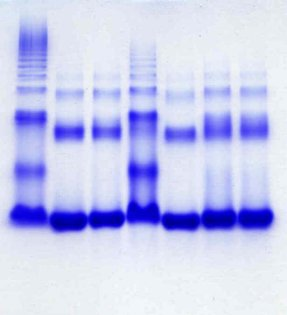
\includegraphics[width=0.35\textwidth]{nativegel}}

\subsection{Native-PAGE 10x Running Buffer}

Dissolve 15.0 g of Tris base, and 72.0 g of glycine in 500 ml of H2O. The pH of the buffer should be 8.3 and no pH adjustment is required. Store the running buffer at room temperature and dilute to 1X before use.

\subsection{Native-PAGE Resolving Buffer}



\begin{table}[ht]
  \centering
  \fontfamily{ppl}\selectfont
  \begin{tabular}{llllll}
    \toprule
    Component & 6\% & 8\% & 10\% & 12\% \\
    \midrule
   30\% Acrylamide		& 2.0 ml & 2.6 ml & 3.4 ml & 4.0 ml \\
   1.5M Tris HCL pH8.8 	& 2.0 ml & 2.0 ml & 2.0 ml & 2.0 ml	\\
    H$_{2}$O 			& 6.0 ml & 5.4 ml & 4.6 ml & 4.0 ml \\

    \bottomrule
  \end{tabular}
  \caption{}
  \label{tab:res}
  %\zsavepos{pos:normaltab}
\end{table}

Store at room temperature in a 10ml Universal. If more than 10 mL store in Duran wrapped in foil to protect from light.


\subsection{Native-PAGE Loading Buffer}

To make 5ml:

\begin{table}[ht]
  \centering
  \fontfamily{ppl}\selectfont
  \begin{tabular}{lll}
    \toprule
    Component & 5x Concentration & Add \\
    \midrule
   100\%Glycerol 		& 50\% 		& 2.5 ml		\\
   0.5M Tris HCl pH 6.8		& 250 mM		& 2.5ml		\\
   Bromophenol Blue		& 0.2\%		& Approximate	\\
   H$_{2}$O 			& 			& up to 5ml	\\

    \bottomrule
  \end{tabular}
  \caption{}
  \label{tab:res}
  %\zsavepos{pos:normaltab}
\end{table}

\newpage
\subsection{Preparing a Gel}

\begin{enumerate}
\item Thoroughly wash glass and combs with water and 70\% isopropanol
\item Mix 5 ml resolving solution, 20 $\mu$L 10\% APS and 5 $\mu$L TEMED per gel in a universal
\item Fill assembled gel (to correct height) and check for leaks
\item Add comb to the gel and leave to dry.
\item Gels are generally ran at 180V. 50 mA (per gel) for 60 min but this can change depending on the experiment.
\end{enumerate}


\chapter{DNA Handling}

\section{Ethanol Precipitation}

\begin{enumerate}
\item Add 1/10th v/v 3M NaAc pH5.2 (1.23g/5ml) to the purified plasmid DNA
\item Add double the volume of ethanol (i.e. 66\% v/v ethanol) and leave on ice for 2 hours (or overnight)
\item Spin at high speed for 30 min
\item Carefully pipette off the supernatant without displacing the pellet
\item Wash the pellet by applying 70\% ethanol and again spin (maintain tube orientation as not to displace the pellet) for a few minutes
\item Carefully pipette off the ethanol and leave to air dry
\item Resuspend the pellet in any volume to concentrate the DNA
\end{enumerate}

\section{Radioactive Substrate Labelling}


\subsection{General Substrate Labelling}

The oligo is 100 uM (therefore 100umoles/L or 100nmoles per mL or 100 pmoles per $\mu$L)


10 fold stock dilution then add 1 $\mu$L (10pMoles) to the 20$\mu$L reaction

Also add:
\begin{itemize}
\item 2$\mu$L 10X PNK buffer
\item 1$\mu$L $\gamma$32P ATP (set concentration)
\item 1$\mu$L T4 PNK enzyme
\item15$\mu$L dH2O
\item 20$\mu$L total
\end{itemize}

\begin{enumerate}
\item Incubate for 2 hours at 37$^{o}$C (in heat block)

\item After 2 hours turn the temperature up to 75$^{o}$C to kill the reaction and leave for30 min

\item Cool reaction on ice for 5 min

\item Use a small gel filtration column (in radioactive lab) pack by spinning at 3000 rpm for 1 min

\item Discard flow through and use a separate eppendorf

\item Add 30 $\mu$L to the 20 $\mu$L reaction (as the optimal volume for the column is 50 $\mu$L. Put onto column and spin for 2 min 3000 rpm

Add another 50$\mu$l H2O to make the total volume 100$\mu$L
\end{enumerate}

The final concentration is 10p moles in 100$\mu$L (assume 100\% recovery) 0.1pmol/$\mu$L which is 0.1$\mu$M


\subsection{Making Annealed Substrates e.g. M13 Oligo Probe}

\begin{enumerate}
\item From a 100$\mu$M stock of oligo do a 1in100 dilution then add 2 $\mu$l of this dilution
\item Also add 2 $\mu$l $\gamma$23P ATP, 1 $\mu$l T4 PNK, 2 $\mu$l T4 PNK buffer (10x) and 13 $\mu$L H2O.
\item Incubate at 37 for 2 hours
\item Heat deactivate at 75 $^{o}$ C for 30 min (use the PCR machine program)
\item Add 12.5 $\mu$l of 1 $\mu$g / $\mu$l M13mp18 (Affymetrix) and then I adjust the total volume to 70 $\mu$l by additing 37.5 $\mu$l milli Q water.
\item Add 3.68 20x SSC buffer\footnote{For \textbf{20x SSC} dissolve 75.3g NaCl and 88.2g of Na$_{3}$ Citrate in 800ml H$_{2}$O. Adjust to pH 7.0 using HCl then adjust the volume to 1L and autoclave. This makes 20x SSC which is 3M NaCl, 300mM Na$_{3}$ Citrate (150mM, 15mM final respectively)} and incubate for 2 min at 90-95 $^{o}$C
\item Switch off the heat block and leave overnight
\item The next day use a microspin column (pack for 1 min at 3,000g then spin mix through for 2 min at 3,000g)
\item Add 126.32 $\mu$l of mQH2O to make vol up to 200 $\mu$l giving us a 10 nM stock
\end{enumerate}



\chapter{Cell Methods}

\section{Making Electrocompetant E.coli}

\begin{enumerate}
\item Thaw a sample of XL1 Blue/BL21 and streak 10$\mu$l onto a plate with relevant resistance. Leave overnight
\item Set up a 10ml starter culture from a single colony. Leave overnight
\item Inoculate 500ml of LB in a baffles glass growth flask, grow at 37$^{o}$C until the optical density at $\lambda$595 reaches 0.7
\item Leave the flask in a cold room (4$^{o}$C) for 30 min to stop growth (PRE-CHILL ALL BOTTLES H2O ETC)
\item Divide the cells into two pre-chilled sterile centrifuge bottles and harvest (3,500 g x 17min at 4$^{o}$C)
\item Wash in 200mL dH2O and harvest (6,000 g x 12min at 4$^{o}$C)\footnote{Washing steps are performed gently but without delay in a 4$^{o}$C cold room with pre-chilled autoclaved dH2O. Resuspension is done by swirling}
\item Repeat step 6
\item Resuspend in 100mL dH2O and harvest (6,000 g x 12min at 4$^{o}$C)
\item Resuspend in 20mL dH2O and divide into two sterile pre-chilled centrifuge tubes. Harvest (6,000 g x 12min at 4$^{o}$C)
\item Resuspend in autoclaved, pre-chilled dH2O (4ml or 6ml for XL1-Blues or BL21 respectively)
\item Snap freeze 80$\mu$l aliquots and store at -80$^{o}$C
\end{enumerate}

\newpage
\section{Electroporation}

Electroporation allows transformation of cells by temporarily creating holes in the cell membrane which allow the passage of charges molecules (in this case plasmid DNA). The physical mechanism involves multiple phases. Phase 1 is a <1 ms 300-400 mV pulse which creates a voltage across the membrane by inducing an ion migration from the surrounding solution. When the critical field is reached a pre-pore forms (a small ($\sim$3�\AA) conductive hydrophobic defect).  Phase 2 involves rearrangements at the pore edge which lead to a hydrophillic interface.

STERILE TECHNIQUE THROUGHOUT

\begin{enumerate}
\item Get the competent cells (XL1 blues/BL21s) out of the fridge (A20 -80) and defrost on ice
\item Get the plasmid sample and defrost on ice (NB the plasmid sample should be around 100 ng/$\mu$l not much above, lower conc. Will be ok just reduce the transformation efficiency)
\item Chill electro cuvetts on ice
\item Set the electroporation machine to Ec2 (this setting is always used unless ligation is being performed)
\item When defrosted put 1 $\mu$l of the plasmid into $\sim$50-85 $\mu$l of competent cells (although one aliquot is usually ok aka 80 $\mu$l). Gently pipette mix up and down with the p100.
\item Leave on ice for 2 min
\item Transfer the mixture into a pre-chilled electrocuvette (Ensure the liquid is touching both plates)
\item Insert the cuvette into the machine making sure its is the correct way round
\item Using the p1000 collect 1 ml of LB
\item Pulse the cells and quickly add the 1ml of LB instantly mixing by pipetting up and down. After a quick mix transfer the sample to labelled eppendorfs
\item Incubate for 1 hour at 37$^{o}$C
\item Inoculate an agar plate with $\sim$250 $\mu$l of the broth(containing relevant plasmid resistance to select for transformants)
\end{enumerate}

\newpage
\section{Glycerol Stocks}

Glycerol stocks are the ultimate long term storage. Plasmids are stored in vivo, the cells are protected by the anti freeze agent glycerol and snap frozen in liquid nitrogen (N2) then stored in a -80 freezer.

\begin{enumerate}
\item Grow a 5ml overnight culture containing all selective antibiotic conditions. \footnote{e.g. pET22b is amp resistant and XL1 blues are tet resistance. The working conc. of tet is 5$\mu$l/ml (therefore 50$\mu$l in 10ml) and amp is 1 $\mu$l/ml (therefore 10$\mu$l in 10 ml) NB amp breaks down after incubated growth so if possible adding half again every $\sim$4 hours is a good idea. Carbenicillin has the same activity as ampicillin but does not break down.}
\item Spin down 10ml to get a pellet (4000rpm 15 min in a fixed angle centrifuge)
\item  Discard the supernatant.
\item  Resuspend the pellet with LB plus 25-50\% glycerol
\item Transfer the suspension into a sterile eppendorf tube. \textbf{Special tubes are available for stocks to be added to the lab strain collection.}
\item Snap freeze the sample in liquid N$_{2}$ \textbf{Undergraduates and masters students must do this under supervision!}
\item Store in the -80 freezer
\end{enumerate}

\chapter{Purification Methods}

\section{TEV Protease}

\subsection{General information}

The TEV protease on this plasmid (pRK793) is a double mutant (L56V/S135G) which reportedly improves solubility and avoids autocatalytic inactivation.

It is expressed in the cell as an MBP-fusion but undergoes self-cleavage to cut off the MBP, creating His-TEV:

GHHHHHHHGESLFKGPRDYNPISSTICHLTNESDGHTTSLYG
IGFGPFIITNKHLFRRNNGTLVVQSLHGVFKVKNTTTLQQHLID
GRDMIIIRMPKDFPPFPQKLKFREPQREERICLVTTNFQTKSM
SSMVSDTSCTFPSGDGIFWKHWIQTKDGQCGSPLVSTRDGF
IVGIHSASNFTNTNNYFTSVPKNFMELLTNQEAQQWVSGWRL
NADSVLWGGHKVFMVKPEEPFQPVKEATQLMNRRRRR

Macrolab purified TEV will cleave 100\% of a control substrate in 2 hr at RT at a molar ratio of 1:50 TEV to substrate (equivalent to 1:125 by mass).

In general, we recommend using TEV at 1:20 by mass, unless you have already tested your substrate and found that you can use less. Some substrates may require significantly more TEV. We do not recommend repeated freeze-thaw cycles. TEV retains full activity for several years when stored at -80$^{o}$C.

TEV is not inhibited by PMSF (1 mM), pepstatin A (1 mM), or complete protease inhibitor cocktail (Roche).


\subsection{Transformation and Expression}

\begin{enumerate}
\item Transform into Rosetta2(DE3)pLysS (other expression strains e.g. BL21 should work but cannot be guaranteed). The plasmid is AmpR, but we use Carbenicillin for selection.
\item Inoculate 2YT (1L) + 100 $\mu$g/ml Carbenicillin with 5 ml of an overnight starter culture.
\item Grow at 37oC to OD of approximately 0.6, induce with 0.5 mM IPTG, and harvest after 2.5 hours of growth at 37$^{o}$C.
\item Pellet cells 4000 rpm 15 mins 4$^{o}$C.
\item Resuspend in 20 ml Nickel A buffer per L cells (25 mM HEPES pH 7.5, 400 mM NaCl, 80 mM imidazole, 10\% glycerol) with 1 $\mu$g/ml leupeptin, 1 $\mu$g/ml pepstatin, 0.5 mM PMSF, 5 mM BME.
\item Freeze cells at -80$^{o}$C.
\end{enumerate}
 
\subsection{Purification(column sizes are for 2L cells)}

\begin{enumerate}
\item Thaw cells and homogenize with 3 passes through Avestin C3 at 10,000-15,000 psi (or sonicate with your own protocol).
\item Clarify lysate 15000 rpm, 30 mins, 4$^{o}$C in SS34.
\item Load lysate onto 5 ml HisTrap FF Crude equilibrated in Nickel A buffer + 5 mM BME.
\item Elute with Nickel B buffer (as for Nickel A but 400 mM imidazole) + 5 mM BME.
\item Desalt into IEX A buffer (25 mM HEPES pH 7.5, 100 mM NaCl, 10\% glycerol) + 5 mM BME. If there is precipitate at this stage, filter the sample (0.2 $\mu$m).
\item Load onto 5 ml HiTrap CaptoS (GE Healthcare) equilibrated in IEX A + 5 mM BME.
\item Elute with step to 100\% IEX B buffer (25 mM HEPES pH 7.5, 400 mM NaCl, 10\% glycerol) + 1 mM DTT.
\item Adjust concentration to 2 mg/ml and freeze in aliquots. Yield is typically 25-30 mg per L.
\end{enumerate}

TEV protease purified by this method is >99\% pure by SDS-PAGE


\appendix

\chapter{Appendix}

\section{Door Codes}


\begin{itemize}

\item Lab A20: 2480x
\item Computer Room: 4568y
\item A Floor Locker Room: 1345y
\item Radioactive Lab: 
\item Radioactive Lab Freezer: 
\item B floor autoclave: 1723x
\item NMR 

\end{itemize}

\section{Useful Websites}

\begin{itemize}
\item Bioinformatic Tools- http://www.ebi.ac.uk/Tools/emboss/
\item Bioinformatic Tool Repository- http://www.expasy.org
\item \textit{E. coli} Genome- http://genolist.pasteur.fr/Colibri/
\item \textit{B. subtilis} Genome- http://genolist.pasteur.fr/SubtiList/
\item Largest Genome Repository- http://www.uniprot.org
\item Human Gene Compendium- http://www.genecards.org
\item Radioactive Ordering- https://workspace.nottingham.ac.uk/display/CBS/Radioisotope+Order+Form
\item HMM Protein Database- http://pfam.xfam.org
\item Database Alignment Tool- http://blast.ncbi.nlm.nih.gov/Blast.cgi
\item Model Threader- http://swissmodel.expasy.org
\item PyMol PDB Viewer- http://pymol.org/educational/
\item US Protein Data Bank- http://www.rcsb.org/pdb/home/home.do
\item EU Protein Data Bank- http://www.ebi.ac.uk/pdbe/
\item SAS Tutorials and Scatter Download- http://www.bioisis.net
\item SAS Discussion Forum- http://www.saxier.org
\item Agresso Ordering- https://agresso.nottingham.ac.uk/
\item MW, pI and Ext Calculator- http://web.expasy.org/protparam/
\item pI Range Calculator- http://protcalc.sourceforge.net


\end{itemize}

\section{Project Codes}


\begin{itemize}
\item Geoff Briggs- RB05EB 
\item Matthew Green- RA05KA \footnote{Currently in use.}
\item Chemistry General Waste Disposal- A10550
\end{itemize}


\section{Extinction Coefficients}

The Extinction coefficient normally quoted is cm$^{-1}$ M$^{-1}$, i.e. a 1 molar solution in a 1 cm cell will give an absorbance of 10930. However, a more useful value is cm$^{-1}$ mg/m$^{-1}$, i.e. a 1 mg/ml solution in a 1 cm cell gives an absorbance of 0.57.

You will notice that if you take the value of 10930 and divide it by the protein MW of $\sim$18000, then you get something close to 0.57. 

%Obviously, if a 1M solution gives an absorbance of 10930, a 1mM solution will give 10.93 and a 100 $\mu$M solution will give 1.1

\begin{table}[ht]
  \centering
  \fontfamily{ppl}\selectfont
  \begin{tabular}{lll}
    \toprule
    Protein & Ext & MW \\
    \midrule
    
\textit{B. subtilis} SSB							& 0.576769	&	 18742.3	\\
\textit{B. subtilis} G23C C51V SSB					& 0.575477	& 	18784.4	\\
\textit {E. coli} SSB								& 1.4693		& 	18975	\\
\textit{B. subtilis} DnaG							& 0.662		& 	68800.4	\\
\textit{B. subtilis} DnaE							& 0.616114	& 	125350	\\
\textit{B. subtilis} his SSB $^{\Delta107-171}$			& 0.583499	&	 14138.8	\\
\textit{B. subtilis} DnaA							& 0.724353	& 	50859.2	\\
\textit{B. subtilis} DnaC							& 0.466578	& 	50602.5	\\
\textit{B. subtilis} DnaD							& 1.24029 	& 	27638.8	\\
\textit{B. subtilis} DnaI 							& 0.653756	&	 36114.4	\\
\textit{B. subtilis} Fully Deuterated SSB				&			&	19992.7	\\
\textit{B. subtilis} PolC							& 0.799		&	162663.3	\\
\textit{B. subtilis} DnaE							& 0.690		&	125349.9	\\


    \bottomrule
  \end{tabular}
  \caption{Extinction coefficients and MW of the proteins currently being used. If your protein is not here but you would like it to be included for easy reference please email matthew.green@nottingham.ac.uk to make a request.}
  \label{tab:res}
  %\zsavepos{pos:normaltab}
\end{table}




\begin{figure}[h]
  \centering
      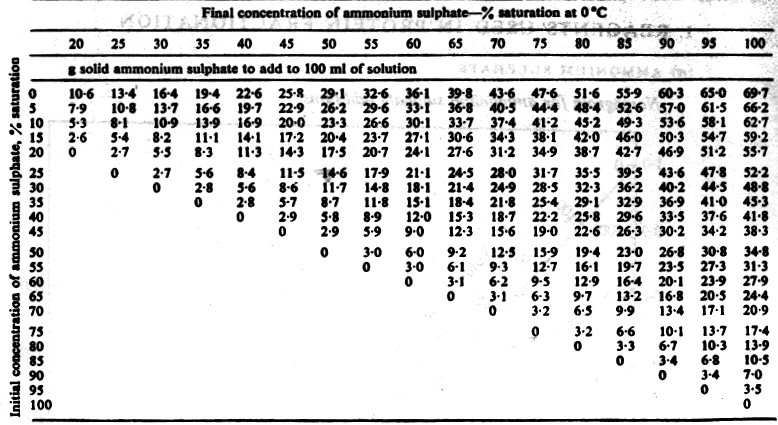
\includegraphics[width=1.0\textwidth]{M1-5}
  \caption{This table is useful for quickly calculating the amount of ammonium sulphate to add to 'cut'. It is especially useful when you already have a solution containing some ammonium sulphate, say 20\%, and you are taking it higher.}
\end{figure}




\begin{figure}[h]
  \centering
      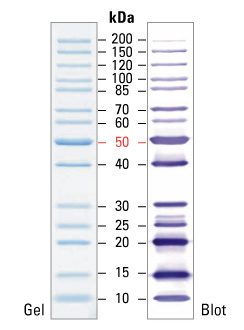
\includegraphics[width=0.5\textwidth]{26614-ladder-002}
  \caption{SDS-PAGE band profile of the Thermo Scientific PageRuler Unstained Protein Ladder. Images represent 8-16\% Tris-glycine gels (SDS-PAGE). Gel was stained with coomassie blue dye; blot was detected with a Strep-Tactin-AP Conjugate and NBT/BCIP substrate.}
\end{figure}






\begin{figure}[h]
  \centering
      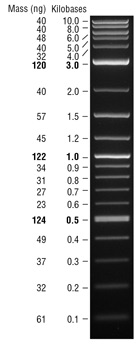
\includegraphics[width=0.35\textwidth]{N3200_thumb}
  \caption{A number of proprietary plasmids are digested to completion with appropriate restriction enzymes to yield 17 bands suitable for use as molecular weight standards for agarose and polyacrylamide gel electrophoresis. The digested DNA includes fragments ranging from 50-1,350 base pairs. The 200 and 500 base pair bands have increased intensity to serve as reference points. 

Comes supplied with 1 vial of Gel Loading Dye, Purple (6X), no SDS. 2-Log DNA Ladder visualized by ethidium bromide staining on a 1.0\% TBE agarose gel. Mass values are for 1 $\mu$g/lane.}
\end{figure}


\begin{figure}[h]
  \centering
      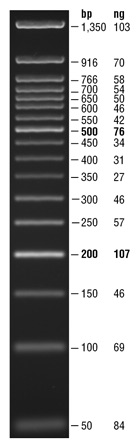
\includegraphics[width=0.35\textwidth]{N3236_thumb}
  \caption{50 bp DNA Ladder visualized by ethidium bromide staining on a 1.8\% TBE agarose gel. Mass values are for 1 $\mu$g/lane.}
\end{figure}





\begin{figure}[h]
  \centering
      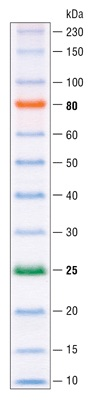
\includegraphics[width=0.35\textwidth]{P7711_thumb}
  \caption{ColorPlus Prestained Protein Ladder, Broad Range (10-230 kDa) is a mixture of highly purified recombinant proteins covalently coupled to a blue dye that resolves into 12 sharp bands when electrophoresed. The protein concentrations are carefully balanced for even intensity. Both the orange 80 kDa and the green 25 kDa bands serve as the reference indicators. The covalent coupling of the dye to the proteins affects their electrophoretic behavior on SDS-PAGE gels relative to unstained proteins (1). The apparent molecular weights of the ColorPlus Prestained Protein Ladder bands were determined on Invitrogen Novex 10�20\% Tris-glycine SDS-PAGE gels (1,2) by comparison to the Protein Ladder. The ColorPlus Prestained Protein Ladder is ideally suited for use in SDS-PAGE and western blotting applications. It allows continuous monitoring of protein separations during electrophoresis and also provides a quick and easy way to assess blotting efficiency (3). 

The ColorPlus Prestained Protein Ladder is designed for use with Tris-glycine gels. 
}
\end{figure}








\end{document}